%Pakete;
%A4, Report, 12pt
\documentclass[ngerman,a4paper,12pt]{scrreprt}
\usepackage[a4paper, right=20mm, left=20mm,top=30mm, bottom=30mm, marginparsep=5mm, marginparwidth=5mm, headheight=7mm, headsep=15mm,footskip=15mm]{geometry}

%Papierausrichtungen
\usepackage{pdflscape}
\usepackage{lscape}

%Deutsche Umlaute, Schriftart, Deutsche Bezeichnungen
\usepackage[utf8]{inputenc}
\usepackage[T1]{fontenc}
\usepackage[ngerman]{babel}

%quellcode
\usepackage{listings}

%tabellen
\usepackage{tabularx}

%listen und aufzählungen
\usepackage{paralist}

%farben
\usepackage[svgnames,table,hyperref]{xcolor}

%font
\usepackage{helvet}
\renewcommand{\familydefault}{\sfdefault}

%Abkürzungsverzeichnisse
\usepackage[printonlyused]{acronym}

%Bilder
\usepackage{graphicx} % Bilder
\usepackage{float}	  %"Floating" Objects, Bilder, Tabellen...

%Pdf einbinden
\usepackage{pdfpages}

%Dokumenteigenschaften
\title{Dkoumentation Simulationsprojekt Hardrock}
\def\author{Reto Schelbert, Simon Schreiber, Tobias Blaser, Urs Baumann}
\providecommand{\teacher}{A. Rinkel}
\providecommand{\room}{5.002}
\providecommand{\versionnumber}{1.2}
\date{\today{}, Rapperswil}


%Kopf- /Fusszeile
\usepackage{fancyhdr}
\usepackage{lastpage}

\pagestyle{fancy}
\fancyhf{} %alle Kopf- und Fußzeilenfelder bereinigen
\fancyhead[L]{System Modelling and Simulation} %Kopfzeile links
\fancyhead[C]{Projekt: Hardrock} %Kopfzeile mitte
\fancyhead[R]{Seite \thepage/\pageref{LastPage}} %Kopfzeile rechts
\renewcommand{\headrulewidth}{0.4pt} %obere Trennlinie
\fancyfoot[L]{\jobname} %Fusszeile links
\fancyfoot[C]{Version: \versionnumber} %Fusszeile mitte
\fancyfoot[R]{\today{}} %Fusszeile rechts
\renewcommand{\footrulewidth}{0.4pt} %untere Trennlinie

%Kopf-/ Fusszeile auf chapter page
\fancypagestyle{plain} {
	\fancyhf{} %alle Kopf- und Fußzeilenfelder bereinigen
	\fancyhead[L]{System Modelling and Simulation} %Kopfzeile links
	\fancyhead[C]{Projekt: Hardrock} %Kopfzeile mitte
	\fancyhead[R]{Seite \thepage/\pageref{LastPage}} %Kopfzeile rechts
	\renewcommand{\headrulewidth}{0.4pt} %obere Trennlinie
	\fancyfoot[L]{\jobname} %Fusszeile links
	\fancyfoot[C]{Version: \versionnumber} %Fusszeile mitte
	\fancyfoot[R]{\today{}} %Fusszeile rechts
	\renewcommand{\footrulewidth}{0.4pt} %untere Trennlinie
}

\usepackage{changepage}

%links, verlinktes Inhaltsverzeichnis, PDF Inhaltsverzeichnis
\usepackage[bookmarks=true,
bookmarksopen=true,
bookmarksnumbered=true,
breaklinks=true,
colorlinks=true,
linkcolor=black,
anchorcolor=black,
citecolor=black,
filecolor=black,
menucolor=black,
pagecolor=black,
urlcolor=black
]{hyperref} % Paket muss unbedingt als letzes eingebunden werden!

\begin{document}

%Titel und Inhaltsverzeichnis
\thispagestyle{empty}
\begin{titlepage}
	\begin{center}

	\vspace*{40mm}
	
	\begin{figure}[htp]
		\centering
		
\includegraphics[width=0.60\textwidth]{img/Hard-Rock-Cafe-Logo-Black-White.png}
	\end{figure}		
	\vspace*{20mm}
	
	{\fontsize{40}{48} \selectfont Projekt Hardrock \\[10mm]}
	{\fontsize{32}{48} \selectfont Dokumentation \\[5mm]}	
	\vspace*{20mm}
	\author

\end{center}
\end{titlepage}
\clearpage

\chapter*{Änderungsnachweis}
\begin{tabularx}{\textwidth}{|cXlr|} % Versionstabelle, Rahmen links und rechts
		\hline
		\textbf{Version} & \textbf{Änderung} & \textbf{Autor} & \textbf{Datum}\\
		\hline
		1.0 & Dokumentenentwurf & Tobias Blaser & 24.03.2013 \\
		1.1 & Entwurf Konzept & Tobias Blaser & 28.03.2013 \\
		1.2 & Ergänzungen und Korrekturen & Reto Schelbert & 03.04.2013 \\
		1.3 & Überarbeitung Konzept (Word Model) & Tobias Blaser & 08.04.2013 \\
		1.4 & Modell \& Verteilungsfunktionen & Tobias Blaser & 03.05.2013 \\
		\hline
\end{tabularx}

% Inhaltsverzeichnis
\tableofcontents


\chapter{Konzept}


\section{Model}
Als Ausgangskonzept wird das Hardrock in Atlantic City verwendet.
\begin{figure}[htp]
	\centering
		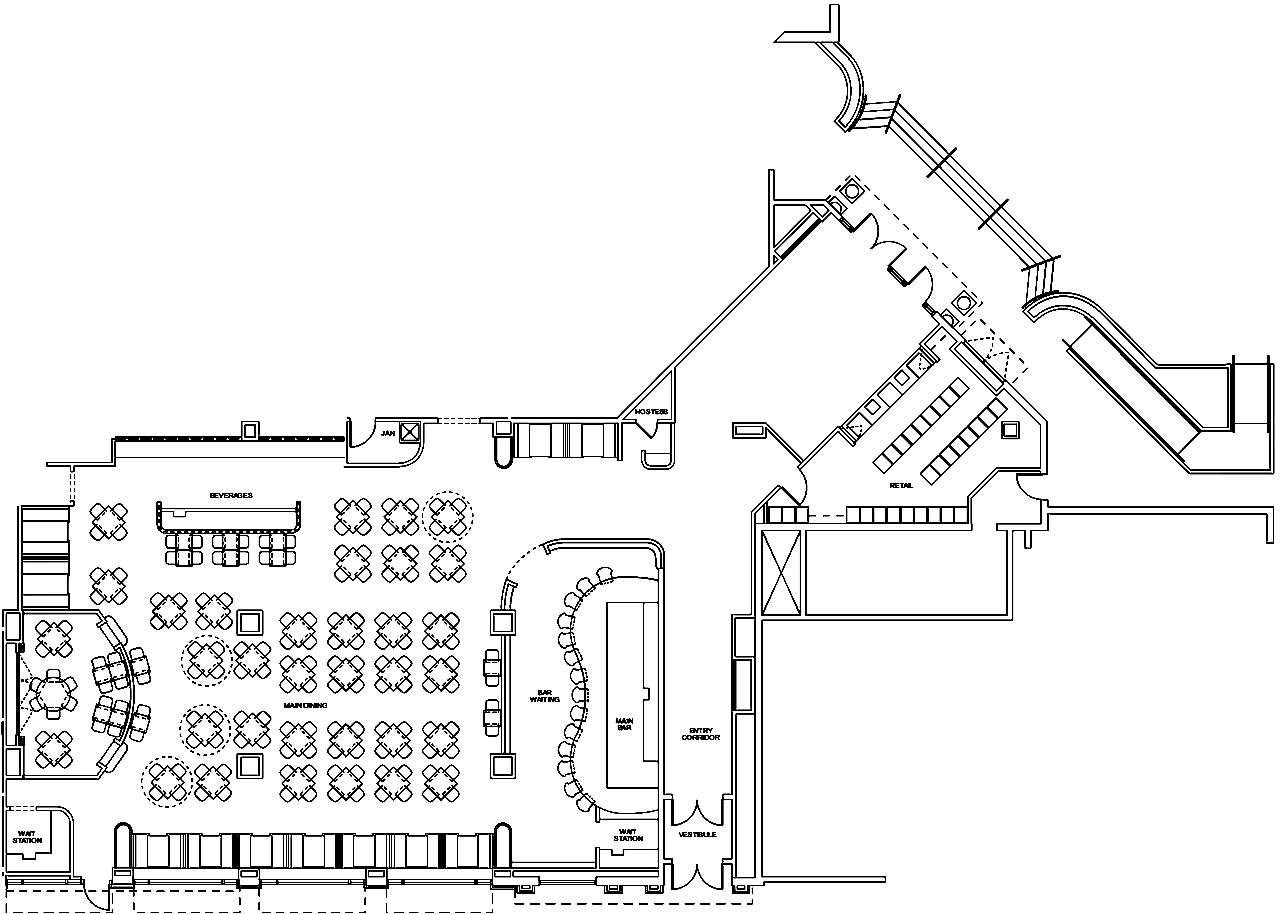
\includegraphics[width=1\textwidth]{img/hardrock-plan.png}
		\caption[Gebäudeplan Hardrock]{Gebäudeplan Hardrock Cafe, Atlantic City (Quelle: www.hardrock.com, 25.03.13)}
		\label{planHardrock}
\end{figure}

\subsection{Eingangsbereich}
Vor dem Eingangsbereich warten die Gäste in einer Schlange, bis an der Bar Plätze frei werden. Die Schlange soll dabei so kurz wie möglich sein. Die Gäste sollen stattdessen an der Bar warten und konsumieren.

\subsection{Bar}
Die Bar dient als Warteschlange an einem Tisch frei werden. Gäste werden an der Bar bedient und konsumieren.
Das Servierpersonal an der Bar soll in unserer Simulation nicht berücksichtigt werden. Grund dafür ist die Unabhängigkeit des Barpersonals vom Rest des Lokals. Das Barersonal geht nicht zwischendurch raus und bedient noch Tische, sondern bedient nur die Gäste an der Bar.

Ziel ist es, dass an der Bar möglichst viele Plätze besetzt sind, weil dies Einnahmen durch Konsumation generiert. Gleichzeitig sollte vor der Türe die Schlange möglichst klein sein oder gar nicht existieren, damit keine Gäste an der Kälte warten müssen, oder sogar wieder gehen. Die Wartezeit an der Bar sollte nicht mehr als ein bis zwei Drinks betragen, damit niemand wieder geht, bevor ein Tisch frei wird.

$\rightarrow$ Annahme Drinklänge: ca. eine Viertelstunde bis 20 Minuten.

\subsection{Tische}
Zu Tisch werden ein bis drei Gänge gegessen. In einem ersten Schritt soll dies sehr einfach abgebildet werden und auf eine komplexe Menüsimulation verzichtet werden.

Das Servierpersonal kommt einmal und bedient. Das Servierpersonal ist somit für eine bestimmte Zeit belegt und anschliessend wieder frei. 

Das Szenario Teller und Karte bringen soll erst in einem zweiten Schritt modelliert werden, je nach verfügbarer Projektzeit.

In der realen Welt bestehen die Tische aus Vierertischen. Ankommenden Gruppen müssen aufgeteilt werden. Oder Tische zusammengeschoben werden. Bei weniger als 4 Personen kann es zu leeren Plätzen kommen. Der Einfachheit halber soll dies nicht berücksichtigt werden in der Simulation.
Die Plätze werden fix gewählt anhand des Beispiels von Atlantic City (250 Plätze).

Nach dem Esssen  verlassen die Gäste das Hardrock und der Tisch wird frei für neue Gäste.
In der Realität kann es durchaus vorkommen, dass Gäste nochmals an die Bar zurückkehren.


\subsection{Küche}
In einem ersten Schritt soll die Küche sehr rudimentär simuliert werden. Es existieren Köche, die eine bestimmte Zeit benötigen, um Essen zuzubereiten. 

In einem Zweiten Schritte könnnten verschiedene Köche, die pro Essen und Gang an eine bestimmte Zeit gebunden sind modelliert werden.

\begin{figure}[H]
	\centering
		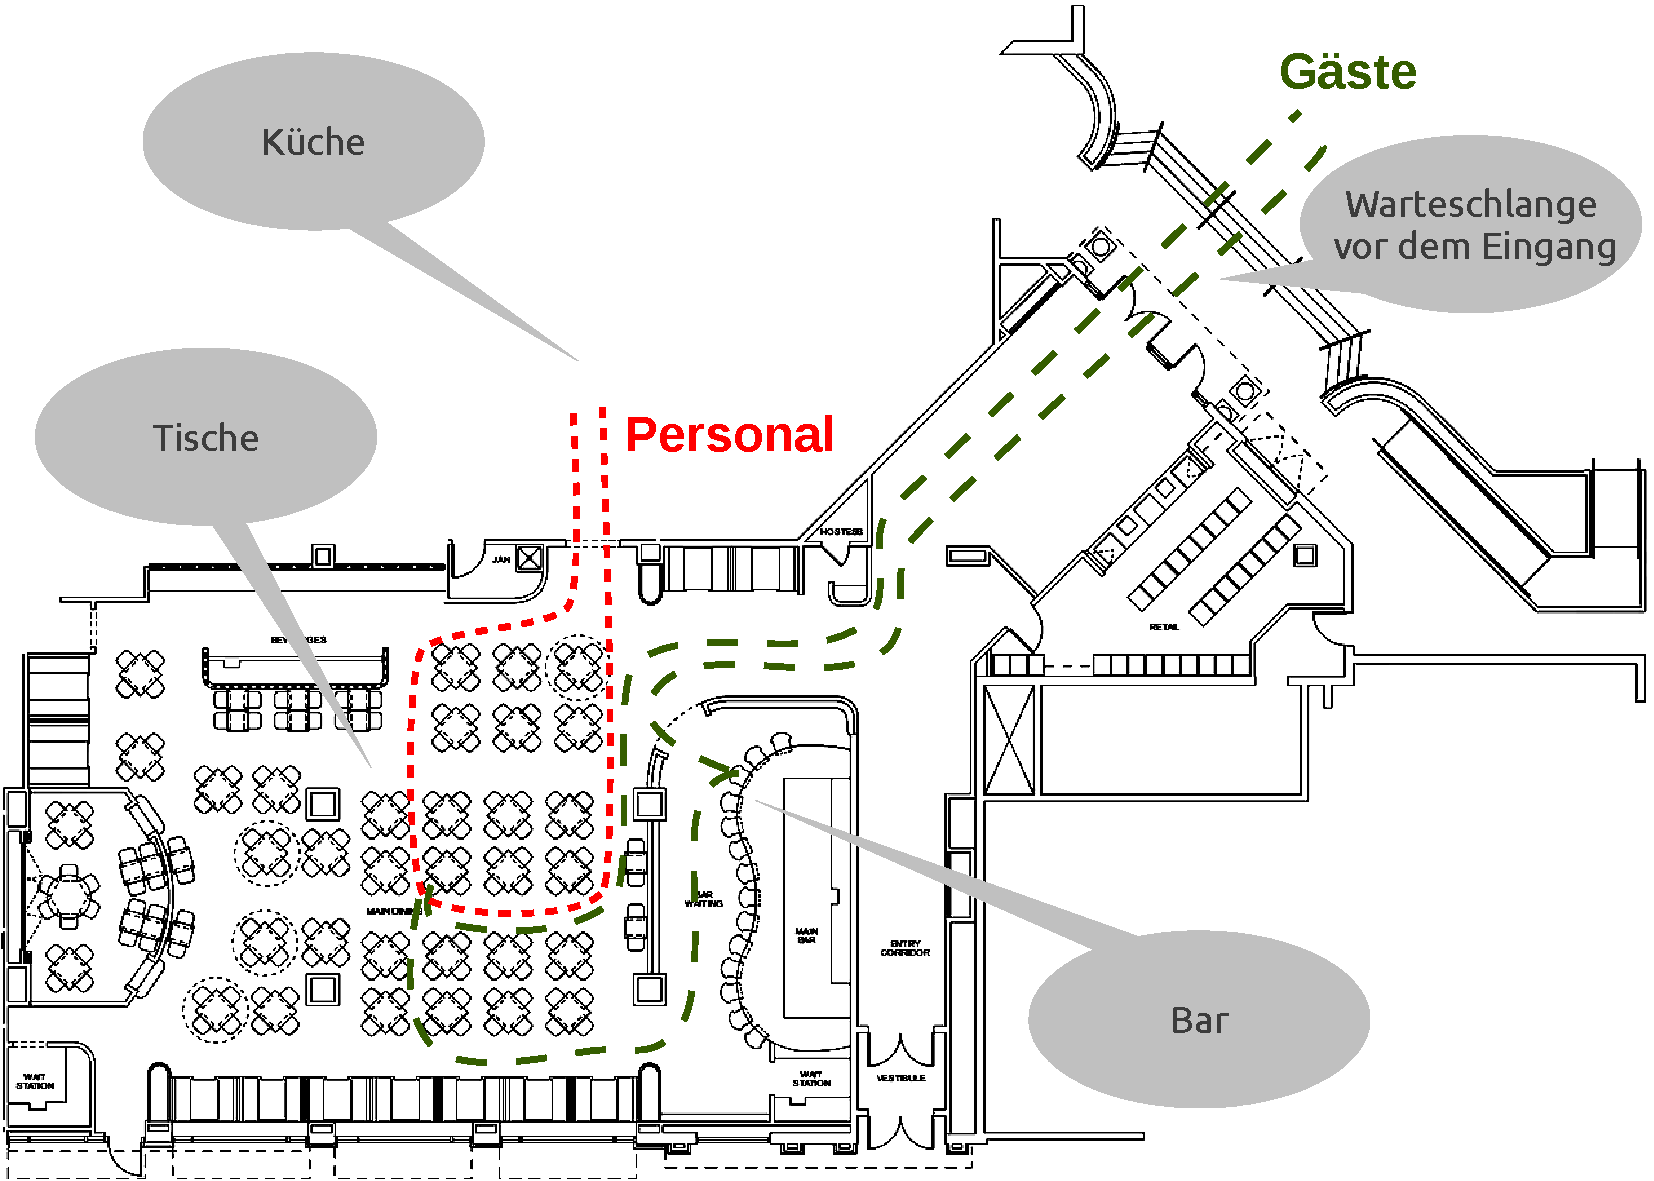
\includegraphics[width=1\textwidth]{img/hardrockSchema.pdf}
		\caption[Bewegungsschema Hardrock]{Bewegungsschema im Hardrock Cafe, Atlantic City}
		\label{schemaHardrock}
\end{figure}



\section{Warum soll Simuliert werden?}
\begin{itemize}
	\item Gebäudebau: Aus Kostengründen ist es nicht möglich einen Prototyp zu bauen
	\item Ist das Gebäude einmal gebaut, so kann die Bar kann nachträglich nur mit grossen Kostenaufwänden vergrössert oder verkleinert werden.
	\item Das Szenario ist zu komplex um alle einfliessenden Faktoren zu berücksichtigen, zu viele Variablen im Spiel sind.
	\item Testen durch Reallife-Simulation ist nicht möglich, weil Statisten beim Warten sterben würden, vom vielen Essen dick würden oder verhungern würden beim Warten auf die Bestellung. Möglicherweise würden Sie auch an der Bar zu viele Drinks nehmen und wären zu betrunken um an einen Tisch zu wechseln.
	\item Zudem tauchen Unsicherheiten auf durch Verteilungen und Verstreuungen und Variabilitäten der Gäste, Serviceagents und deren Servicetime, Warteschlangen und Wartezeiten.
\end{itemize}

\section{Objectives}
\begin{itemize}
	\item Vor der Türe:
		\begin{itemize}
			\item Queue: Ankommende Gäste lim(0)
		\end{itemize}
	\item Küche
		\begin{itemize}
			\item Agents: Köche
		\end{itemize}
	\item Bedienung
		\begin{itemize}
			\item Agents: Kellner, Tellerbringer
		\end{itemize}
	\item Bar
		\begin{itemize}
			\item Queue: Anzahl Warteplätze
		\end{itemize}
	\item Tische
		\begin{itemize}
			\item Ressourcen: Anzahl Plätze
		\end{itemize}
\end{itemize}



\section{Fragestellungen}
Ziel ist die Gewinnmaximierung durch gute Auslastung. Als gute Auslastung wird 75\% Utilisation angenommen.
\subsection{Grösse der Bar}
\textbf{Wie viele Plätze muss die Bar bieten, damit fast keine Gäste in der Kälte vor dem Eingang warten müssen und die mittlere Aufenthaltszeit an der Bar ein bis zwei Drinks nicht übersteigt?} \\
Als Länge für einen Drink soll 15-20 Minuten angenommen werden.


\subsection{Benötigtes Personal}
\textbf{Wie viel Servierpersonal und wie viele Köche braucht es, damit die Mittlere Aufenthaltszeit am Tisch bei ca. 1.5 Stunden liegt, und die mittlere Wartezeit ca. 15 Minuten nicht übersteigt?} \\


\section{Spezifikationen}
Gearbeitet wird mit Fiktiven Daten, ausgenommen die Anzahl der Plätze im Saal. Diese werden vom Hardrock Atlantic City übernommen.

\subsection{Variable Grössen}
Es sollen verschiedene Szenarien simuliert werden. Die dazu benötigten Grössen sollen Variabel sein:
\begin{itemize}
	\item Queuelänge
	\item Anzahl Servierpersonal
	\item Anzahl Köche
	\item Gruppen mit unterschiedlichen Anzahlen von Gästen
\end{itemize}

\subsection{Resultatgrössen}
Durch die Simulation sollen die \textbf{Aufenthaltszeiten an der Bar (Queue)}, die \textbf{Dauer des Aufenthaltes und Wartezeiten am Tisch}, die \textbf{Gesammtaufenthaltsdauer im Restaurant} und die \textbf{Auslastung der Agenten} ermittelt werden

\subsection{Zusatzprojekt (optional)}
In einem weiteren Projekt kann die Simulation ausgebaut und verfeinert werden, indem weitere Parameter hinzugefügt  und detailliertere Daten erhoben werden:
\begin{itemize}
	\item Anzahl Personal an der Bar
	\item Verschiedene Essen/Menüs mit unterschiedlichen Servicezeiten für die Köche.
	\item Anzahl Tellerbringer
	\item Gruppen müssen zusammen an einem Tisch untergebracht werden, keine Leerplätze.
	\item Weitere Resultate: Wie lange dauert die Bestellaufnahme, wie lange muss ein Gast durchschnittlich auf die Bestellung warten und wie lange wartet er auf die Rechnung? Wie oft muss das Servicepersonal an einen Tisch gehen pro Gast?
	\item Optional: Animation
\end{itemize}


\chapter{Modellierung}
	\section{Activities}
		\begin{figure}[H]
			\centering
				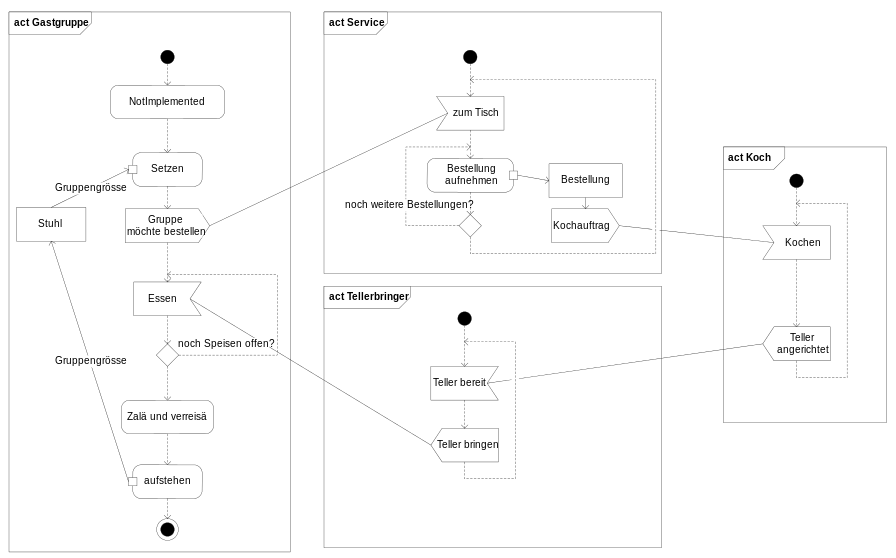
\includegraphics[width=1\textwidth]{img/activityDiagramm-v1.png}
				\caption[Activity Diagramm]{Activity Diagramm}
				\label{activityDiagramm}
		\end{figure}
		
		\subsection{Gastgruppe}
		
		\subsection{Service}
		
		\subsection{Tellerbringer}
		
		\subsection{Koch}
		

\begin{landscape}
	\section{Hardrock Flow}
		\begin{figure}[H]
			\centering
				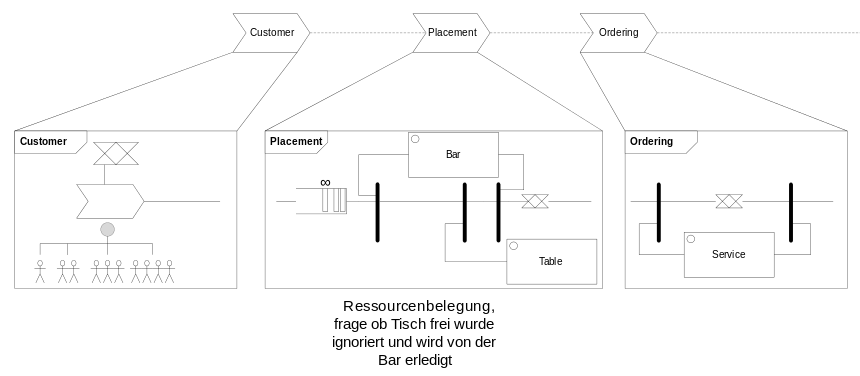
\includegraphics[width=1.4\textwidth]{img/flowDiagramm1-v1.png}
				\caption[Hardrock Flow Diagramm Teil1]{Hardrock Flow Diagramm Teil1}
				\label{flowDiagramm1}
		\end{figure}
		
		\subsection{Customer}
		
		\subsection{Placement}
		
		\subsection{Ordering}
		
		
		\begin{figure}[H]
				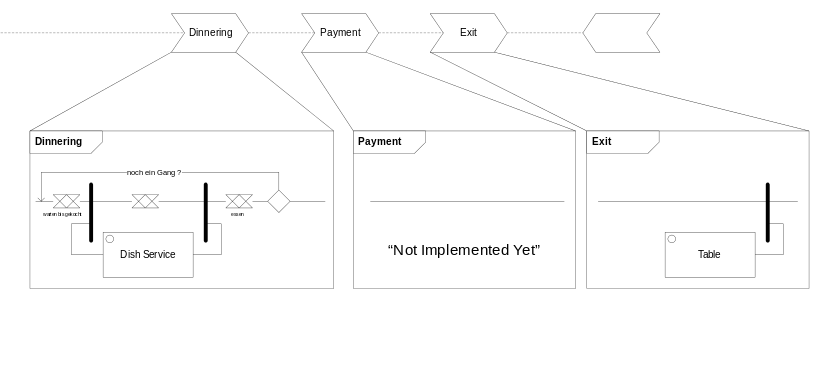
\includegraphics[width=1.4\textwidth]{img/flowDiagramm2-v1.png}
				\caption[Hardrock Flow Diagramm Teil2]{Hardrock Flow Diagramm Teil2}
				\label{flowDiagramm2}
		\end{figure}
		
		\subsection{Dinnering}
		
		\subsection{Payment}
		
		\subsection{Exit}
		
		
\end{landscape}



\chapter{Simulation}
	\section{Verteilung der ankommenden Gäste}
	Um die Verteilung des Andrangs und die beiden Spitzenzeiten zu simulieren, nutzen wir einen Scedule.
	Der Sceduler erzeugt eine negative Exponentialverteilung.
	
	\section{Verteilung der Zubereitungszeit}
	Für die Verteilung der Kochzeit wählen wir eine Mormalverteilung mit einem Mittelwert von fünf und einer Standardabweichung von drei Minuten.
	
	Da im Hardrock verschiedenste Speisen zubereitet werden, von Salaten über Hauptgängen bis Deserts, ist Normalverteilung hier die sinnvollste Abbildung.
	
	\section{Gruppenbestellungen}
	Gruppen bestellen gemeinsam, erhalten ihr Essen gemeinsam, gekocht wird es jedoch unabhängig. Dazu wird die Bestellung dupliziert und damit in der Küche vier Unterbestellungen simuliert. Vor dem Servieren werden die Bestellungen wieder zu einer gesammtbestellung zusammengefügt.

\chapter{Auswertung}



\appendix
\chapter{Präsentation Projektvorstellung}
\includepdf[pages=1-3,angle=180, scale=0.9]{media/presentation-hardrock-slides.pdf}

\listoffigures

\chapter{Materialnachweise}
\section{Titelblatt}
\begin{tabularx}{\textwidth}{|Xlr|}
		\hline
		Logo Hardrock & www.hardrock.com & 25.03.2013 \\
		\hline
\end{tabularx}

\end{document}
